\section{GVNS+: Enhanced baseline metaheuristic framework}
\label{sec:baseline}

\subsection{Original GVNS framework}
The foundation of the proposed framework is the Generalized Variable Neighborhood Search (GVNS) algorithm recently introduced by \citet{masmoudi2025generalized}, which currently represents one of the most competitive metaheuristic approaches for the Vehicle Routing Problem with Time Windows and Synchronization constraints (VRPTW-S).

The method combines diversification and intensification mechanisms through three main components. First, a shaking phase applies progressively stronger perturbations to escape local optima and diversify the search trajectory. Second, a Variable Neighborhood Descent (VND) procedure explores a sequence of neighborhood structures in order to intensify the search around promising solutions. Finally, an adaptive acceptance mechanism allows the algorithm to temporarily explore infeasible regions while dynamically regulating the penalties associated with synchronization and temporal violations.

A major strength of the GVNS lies in its ability to efficiently balance exploration and exploitation in highly constrained synchronized routing problems. By combining multiple neighborhood structures with adaptive penalty management, the method achieved state-of-the-art performance on the benchmark instances introduced by \citet{bredstrom2008combined} and later extended by \citet{liu2019adaptive}, establishing numerous best-known solutions \citep{masmoudi2025generalized}.

For these reasons, GVNS was selected as the optimization backbone of the present study. Rather than replacing the underlying metaheuristic, our objective is to strengthen its search capabilities and subsequently investigate how learning-based mechanisms can further improve its adaptive behavior.

\subsection{Added neighborhood operators}
Although the original GVNS exhibits strong performance, the present work required a robust and scalable implementation capable of supporting subsequent learning-based extensions. During the initial Python reimplementation of the original framework, a noticeable performance gap remained with respect to the reference C++ implementation reported in the literature. To strengthen the optimization backbone before introducing adaptive mechanisms, the neighborhood portfolio was extended through the integration of four additional operators.

The original framework relies on four classical neighborhoods based on relocation and exchange moves performed either within a route or between routes. To complement these local modifications, four larger-scale operators were incorporated: Cross-Exchange, $k$-Relocate, 2-Opt, and 2-Opt*.

Cross-Exchange simultaneously swaps route segments between two different routes, enabling substantial route restructuring. The $k$-Relocate operator transfers consecutive customer sequences rather than individual visits, allowing larger route modifications in a single move. The 2-Opt operator reverses route segments within a route to eliminate inefficient crossings and improve route geometry, while 2-Opt* exchanges route tails between two routes and has proven particularly effective in vehicle routing applications.

These operators were selected because of their demonstrated effectiveness in routing literature and their complementary exploration behavior \citep{liu2019adaptive}. Whereas the original neighborhoods mainly perform localized modifications, the additional operators enable larger structural transformations capable of escaping deeper local optima. The resulting framework, denoted GVNS+, preserves the overall architecture of the original algorithm while providing a richer neighborhood portfolio and enhanced search diversification capabilities.

\subsection{Large-scale benchmark generation}
Existing VRPTW-S benchmark sets provide valuable evaluation references but remain relatively limited in scale for studying adaptive optimization mechanisms. The benchmark proposed by \citet{bredstrom2008combined} contains instances derived from Solomon problems with up to 80 customers, while the larger dataset introduced by \citet{liu2019adaptive} extends problem sizes to 200 customers.

Such benchmarks are sufficient for evaluating conventional metaheuristics but provide limited opportunities for assessing scalability and learning generalization. Since the objective of this work is to investigate adaptive search mechanisms, a broader set of optimization scenarios was required.

To address this limitation, a new family of synchronized VRPTW-S instances was generated from the classical Solomon benchmark. The original customer coordinates, demands, service durations, vehicle capacities, and time-window characteristics were preserved in order to maintain the structural properties of the underlying VRPTW instances. Synchronization constraints were then introduced by creating pairs of customers requiring simultaneous service.

Four instance sizes were considered: 50, 100, 200, and 400 customers. The first two correspond to commonly used benchmark sizes, whereas the latter two significantly extend the scale of synchronized routing problems considered in the literature. For each size category, 56 synchronized instances were generated, resulting in a total collection of 224 benchmark instances.

To maintain a comparable workload across instance sizes, fleet sizes were scaled proportionally with the number of customers. Instances containing 50 and 100 customers were assigned 25 vehicles, 200-customer instances used 50 vehicles, and 400-customer instances employed 100 vehicles. Similarly, synchronization density was preserved by introducing 5, 10, 20, and 40 synchronized customers for the four size categories respectively.

Following the construction principles adopted in existing synchronized benchmarks, synchronization constraints were preferentially assigned to customers possessing relatively wide time windows. This strategy increases the likelihood of generating feasible synchronized services while preserving the routing complexity induced by temporal coordination.

The resulting benchmark extends existing VRPTW-S datasets both in scale and complexity and serves as the primary experimental environment for evaluating the adaptive mechanisms proposed in this paper.

\subsection{Learning Infrastructure and Search-State Representation}
The adaptive mechanisms introduced later in this work require the ability to observe and characterize the current optimization context. Unlike conventional machine learning applications, no training dataset exists a priori for the VRPTW-S. The information required by the learning models must therefore be generated directly from the execution of the optimization algorithm itself. To address this challenge, a unified learning infrastructure was integrated into GVNS+, enabling the continuous observation of the search process and the construction of datasets suitable for the different adaptive components investigated in this study.

Figure~\ref{fig:data_collection_pipeline} summarizes the overall data collection process. Starting from repeated executions of GVNS+ on the training benchmark instances, the framework successively performs search-state extraction, trajectory logging, offline dataset construction, and task-specific preprocessing before producing the final datasets used by the learning models.

\begin{figure}[ht]
\centering
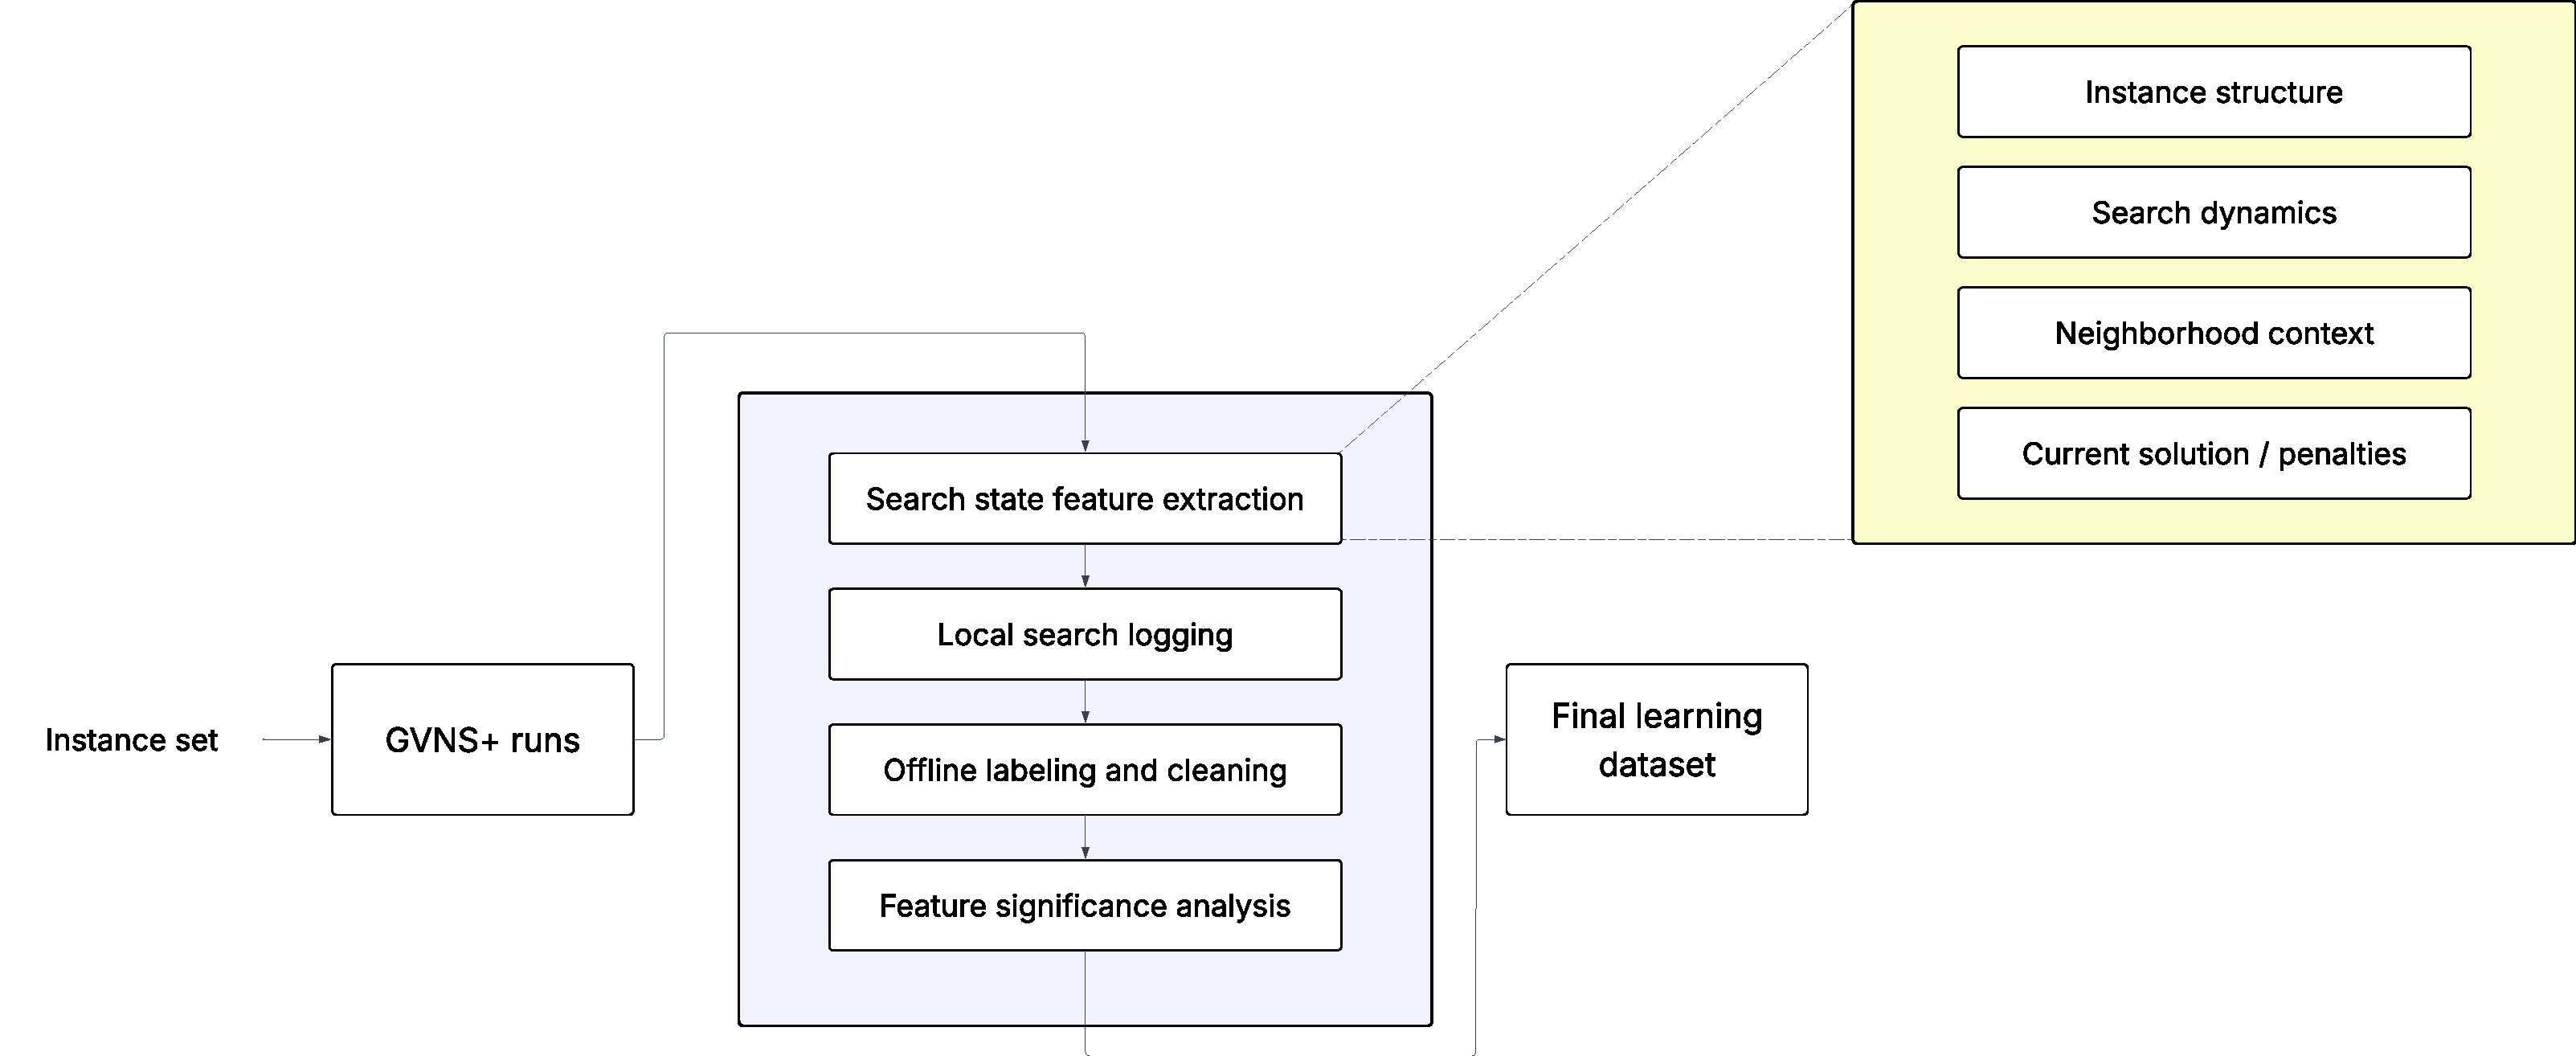
\includegraphics[width=\linewidth]
{../figures/data_collection_pipeline.pdf}

\caption{Data collection pipeline for learning-based adaptation}
\label{fig:data_collection_pipeline}
\end{figure}

Since complete routing solutions are high-dimensional and computationally expensive to process directly, the optimization state is represented through a compact set of descriptors summarizing the current search situation. The proposed representation combines four complementary categories of features.

Instance-level descriptors characterize the solved problem through information such as instance size, fleet size, synchronization density, planning horizon, and time-window characteristics. These features remain constant during a run and provide contextual information regarding the difficulty and structure of the optimization instance.

Dynamic search descriptors capture the evolution of the optimization process over time. They include indicators related to iteration progress, search stagnation, recent improvement rates, and the evolution of solution quality over a rolling observation window. These features provide information about whether the search is actively progressing or entering a stagnation phase.

Solution-structure descriptors summarize the current routing solution through lightweight indicators reflecting route organization and feasibility pressure. Examples include route-balance measures, waiting-time statistics, lateness indicators, and penalty-related information. Such descriptors provide an approximate characterization of solution quality while remaining computationally inexpensive.

Finally, neighborhood-context descriptors characterize the local search environment by recording information related to the active neighborhood operator and its recent behavior. These descriptors allow the adaptive models to distinguish decisions occurring under different exploration conditions.

To generate learning data, GVNS+ was executed repeatedly on the training benchmark instances. During each run, the search-state descriptors were continuously recorded together with the corresponding optimization decisions and their outcomes. Because the metaheuristic contains stochastic components, repeated executions of the same instance naturally generate diverse optimization trajectories, exposing the learning models to a wide range of search situations, including productive improvement phases, neighborhood transitions, and prolonged stagnation periods.

The collected logs were subsequently processed offline to construct task-specific learning datasets. Depending on the considered adaptive mechanism, additional labels, rewards, or decision targets were derived from the recorded optimization outcomes. Basic preprocessing operations, including duplicate filtering, removal of non-informative variables, and feature-correlation analysis, were applied to reduce redundancy while preserving the most relevant information for each learning task.

The resulting infrastructure provides a common data foundation for all adaptive components developed in this work. Although the learning objectives differ across reinforcement learning, supervised learning, and policy-learning approaches, all models operate from the same unified representation of the search process, ensuring consistency while maintaining a compact and computationally efficient description of the optimization context.
\subsection{Validation against literature benchmarks}
Before introducing learning-based adaptations, the performance of GVNS+ was evaluated on the benchmark instances commonly used in the VRPTW-S literature. The objective was to verify that the proposed enhancements preserve the effectiveness of the original method while reducing the performance gap introduced during the Python reimplementation.

The validation experiments were conducted on the benchmark instances of \citet{bredstrom2008combined} and \citet{liu2019adaptive}, using the same evaluation protocol adopted by \citet{masmoudi2025generalized}. The obtained solutions were compared against the best-known results reported in the literature.

The integration of the additional neighborhood operators substantially improved solution quality across all benchmark categories. Whereas the initial reimplementation exhibited an average performance gap of approximately 10\% relative to the reference implementation, the enhanced GVNS+ reduced this gap to 1.14\% on average. Furthermore, the method remained highly competitive with respect to published state-of-the-art results while preserving reasonable computational times.

These results confirm that the proposed enhancements successfully strengthen the optimization backbone without altering the fundamental search principles of the original GVNS. Consequently, GVNS+ provides a reliable and competitive baseline from which the impact of the subsequent learning-guided adaptations can be assessed.
